\clearpage

\section{Timing Deskew}

\begin{tcolorbox}	
	\begin{tabular}{p{2.75cm} p{0.2cm} p{10.5cm}} 	
		\textbf{Header File}   &:& timing\_deskew.h \\
		\textbf{Source File}   &:& timing\_deskew.cpp \\
        \textbf{Version}       &:& 20190225 (Daniel Pereira)\\
	\end{tabular}
\end{tcolorbox}

This block allows for the removal of the timing mismatches between the real and imaginary components of a complex signal.

\subsection*{Input Parameters}

\begin{table}[h]
	\centering
	\begin{tabular}{|c|c|p{60mm}|c|ccc}
		\cline{1-4}
		\textbf{Parameter} & \textbf{Type} & \textbf{Values} & \textbf{Default}  \\ \cline{1-4}
		skew     & vector<\texttt{double}> & any             & [0, 0]            \\ \cline{1-4}
	\end{tabular}
	\caption{Timing deskew input parameters} 
	\label{table:TimingDeskew_in_par}
\end{table}

\subsection*{Methods}

\bigbreak
TimingDeskew(initializer\_list$<$Signal *$>$ \&InputSig, initializer\_list$<$Signal *$>$ \&OutputSig) :Block(InputSig, OutputSig)\{\};
\bigbreak
void initialize(void);
\bigbreak
bool runBlock(void);
\bigbreak
void setSkew(vector<double> s) \{ skew.resize(s.size()); skew[0] = s[0]; skew[1] = s[1]; \}

\subsection*{Functional description}

This DSP step takes a complex input signal and removes a given amount of timing skew between its real (in-phase) and imaginary (quadrature) parts. This DSP step follows the topology presented in Figure~\ref{fig:mqamDiagramDSP_DS},
%
\begin{figure}[h]
\centering
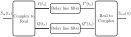
\includegraphics[scale=1]{./lib/timing_deskew/figures/diagramDSP_DS}
\caption{Block diagram representation of the deskew procedure.}
\label{fig:mqamDiagramDSP_DS}
\end{figure}
%
in which the input signal $S_\text{in}(n)$ is separated into its in-phase and in-quadrature components, $I(n)$ and $Q(n)$ and are each sent through independent delay line filters. In turn, the delay line filters function as shown in Figure~\ref{fig:mqamDiagramDSP_DL}.
%
\begin{figure}[h]
\centering
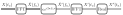
\includegraphics[scale=1]{./lib/timing_deskew/figures/diagramDSP_DL}
\caption{Block diagram representation of the implemented delay line filter.}
\label{fig:mqamDiagramDSP_DL}
\end{figure}
%
The signal at the input, $S_\text{in}(t_n)$, is transformed to Fourier space, where it is multiplied by a deskew element $\tau$
%
\begin{align}
\hat{S}^\prime(f_n)&=\hat{S}(f_n) e^{i2\pi f_n \tau}.
\end{align}
The value of $\tau$ here is set by trial and error and is characteristic of a certain receiver. For these results the timing skew was set at 20~ps.
\par
This signal is then transformed back to time domain and the imaginary part is discarded. After both components are passed through the delay line, they are combined into a complex signal as the output

\begin{equation}
S_\text{out}(t_n)=\text{real}(I^{\prime\prime}(t_n))+i\text{real}(Q^{\prime\prime}(t_n)).
\end{equation}

\subsection*{Input Signals}

\textbf{Number:} 1\\
\textbf{Type:} Complex signal

\subsection*{Output Signals}

\textbf{Number:} 1\\
\textbf{Type:} Complex signal

